\chapter{Metodologia}

Esta seção apresenta os procedimentos adotados para o desenvolvimento, a implementação e a validação técnica da interface musical multissensorial proposta.

A metodologia foi organizada de forma incremental, iniciando pelo dimensionamento e pela simulação do circuito eletrônico de acionamento, seguida pela implementação da lógica computacional, configuração da comunicação entre o computador e o sistema embarcado e integração progressiva dos diferentes módulos do protótipo.

Após a validação inicial em bancada, foi realizada uma etapa adicional de integração destinada à transformação do circuito experimental em uma unidade vestível com alimentação própria. Nessa etapa foram incorporados o sistema de alimentação por baterias, o estágio de regulação de tensão e o LED de alto brilho utilizado como modalidade física complementar de feedback visual.

Os procedimentos experimentais abrangeram a aquisição das mensagens MIDI, o mapeamento entre o parâmetro \textit{velocity} e os valores PWM, a comunicação UDP, o estágio eletrônico de acionamento, a alimentação embarcada, o funcionamento dos canais tátil e visual e a operação integrada da arquitetura.

Os resultados obtidos a partir desses procedimentos são apresentados e discutidos no Capítulo 5.

\section{Estratégia Geral de Desenvolvimento}
\markright{Metodologia}
\label{sec:estrategia_desenvolvimento}

O desenvolvimento foi organizado em etapas modulares: definição dos requisitos de aquisição MIDI e resposta multissensorial, dimensionamento e simulação do circuito de acionamento, implementação do software e da comunicação UDP, testes de bancada e integração dos módulos em uma unidade vestível.

Os componentes eletrônicos foram avaliados inicialmente de forma independente, com verificação do estágio de chaveamento antes da conexão do motor. Posteriormente foram incorporados o canal visual, a alimentação por baterias e o invólucro. Essa sequência permitiu identificar problemas de montagem antes da operação integrada.

Os ensaios utilizaram registros dos programas Python, do monitor serial do ESP32, arquivos CSV e medições elétricas. Os procedimentos específicos são descritos nas seções seguintes.

\subsection{Componentes de Hardware}
\markright{Metodologia}
\label{sec:componentes_hardware}

A Tabela~\ref{tab:componentes_hardware} reúne os componentes principais da configuração final.

\begin{table}[htbp]
\centering
\caption{Principais componentes de hardware utilizados no sistema}
\label{tab:componentes_hardware}
\footnotesize
\begin{tabular}{|p{2.8cm}|p{2.8cm}|c|p{6.8cm}|}
\hline
\textbf{Componente} &
\textbf{Modelo / especificação} &
\textbf{Qtd.} &
\textbf{Função no sistema} \\
\hline
Controlador MIDI & Akai MPD218 & 1 &
Geração das mensagens MIDI a partir da interação com os \textit{pads}. \\
\hline
Microcontrolador & ESP32-WROOM-32 (placa de desenvolvimento) & 1 &
Recepção dos comandos via Wi-Fi/UDP e controle das saídas. \\
\hline
Motor vibrotátil & Vibracall 1027 & 1 &
Produção do \textit{feedback} vibrotátil. \\
\hline
Transistor MOSFET & IRLZ44N & 1 &
Chaveamento da corrente do motor a partir do sinal de controle. \\
\hline
Diodo de proteção & 1N5819 & 1 &
Recirculação da corrente indutiva durante o desligamento do motor. \\
\hline
Resistor de \textit{gate} & 220~$\Omega$ & 1 &
Limitação da corrente transitória associada ao acionamento do \textit{gate}. \\
\hline
Resistor \textit{pull-down} & 47~k$\Omega$ & 1 &
Manutenção do MOSFET no estado desligado sem comando ativo. \\
\hline
LED de alto brilho & -- & 1 &
Produção do \textit{feedback} visual. \\
\hline
Resistor do LED & 220~$\Omega$ & 1 &
Limitação da corrente no LED. \\
\hline
Baterias recarregáveis & Li-ion 18650, 3,7~V & 2 &
Fornecimento de energia à unidade vestível em configuração 2S. \\
\hline
Sistema de proteção & BMS 2S & 1 &
Proteção do conjunto de baterias. \\
\hline
Conversor DC--DC & MP1584EN & 1 &
Redução e ajuste da tensão para aproximadamente 3,3~V. \\
\hline
Computador & Uso geral & 1 &
Aquisição MIDI, interface gráfica, cálculo do comando e transmissão UDP. \\
\hline
\end{tabular}
\legend{Fonte: Elaboração própria (2026).}
\end{table}

Os componentes foram selecionados para atender às funções de aquisição, processamento, comunicação e atuação com disponibilidade comercial e simplicidade de reprodução. O dimensionamento dos resistores, a escolha do estágio de proteção e a estratégia de alimentação são detalhados na Seção~\ref{sec:dimensionamento_circuito}.

\section{Dimensionamento do Circuito Eletrônico}
\markright{Metodologia}
\label{sec:dimensionamento_circuito}


O circuito eletrônico de acionamento foi dimensionado para permitir o controle do motor vibrotátil a partir do sinal PWM gerado pelo microcontrolador ESP32, evitando que a corrente necessária ao atuador seja fornecida diretamente pelo pino GPIO.

O dimensionamento considerou as limitações das saídas do microcontrolador, o comportamento indutivo do motor de corrente contínua, os transitórios associados ao chaveamento PWM e a necessidade de proteção do estágio eletrônico.

A configuração final utiliza um canal de acionamento vibrotátil baseado em transistor MOSFET de canal N. O canal visual é controlado por uma saída independente do ESP32 e utiliza um LED de alto brilho conectado por meio de resistor limitador de corrente.

Embora as duas modalidades possuam circuitos de saída distintos, o mesmo valor PWM calculado a partir do parâmetro \textit{velocity} é utilizado como referência para o acionamento do motor e do LED.

\subsection{Circuito Eletrônico de Acionamento}
\markright{Metodologia}
\label{sec:implementacao_eletronica}

O estágio vibrotátil foi implementado com um MOSFET IRLZ44N de canal N em configuração \textit{low-side}. O terminal positivo do motor é conectado ao barramento regulado, o terminal negativo ao \textit{drain} do MOSFET e o \textit{source} ao GND. O sinal PWM do GPIO 18 é aplicado ao \textit{gate} por um resistor de 220~$\Omega$, e um resistor de 47~k$\Omega$ mantém o transistor desligado quando o pino de controle não está ativamente polarizado.

O IRLZ44N é classificado pelo fabricante como MOSFET de nível lógico, mas seus valores garantidos de resistência de condução são especificados para tensões de \textit{gate} superiores à alimentação lógica utilizada neste protótipo \cite{infineonirlz44n}. Por essa razão, não se assume saturação plena a 3,3~V. A adequação do componente, nas condições empregadas e com a corrente reduzida do motor, foi incluída nos ensaios de validação funcional.

O motor apresenta comportamento indutivo. Um diodo Schottky 1N5819 foi conectado em paralelo ao atuador, polarizado reversamente durante a condução normal, para fornecer caminho de recirculação à corrente no desligamento \cite{vishay1n5819}. A influência dessa proteção é analisada nas simulações da Seção~\ref{sec:simulacao_circuito}.

O canal visual é eletricamente independente do estágio com MOSFET. O LED de alto brilho é conectado ao GPIO 21 em série com um resistor de 220~$\Omega$. Não foram empregados capacitores de desacoplamento adicionais nem fusível resetável PTC na montagem final descrita nesta monografia.

A Figura~\ref{fig:esquematico_canais_saida} apresenta o esquema elétrico dos canais de saída, incluindo o estágio de acionamento do motor, o diodo de proteção e o canal visual.

\begin{figure}[!htbp]
\centering
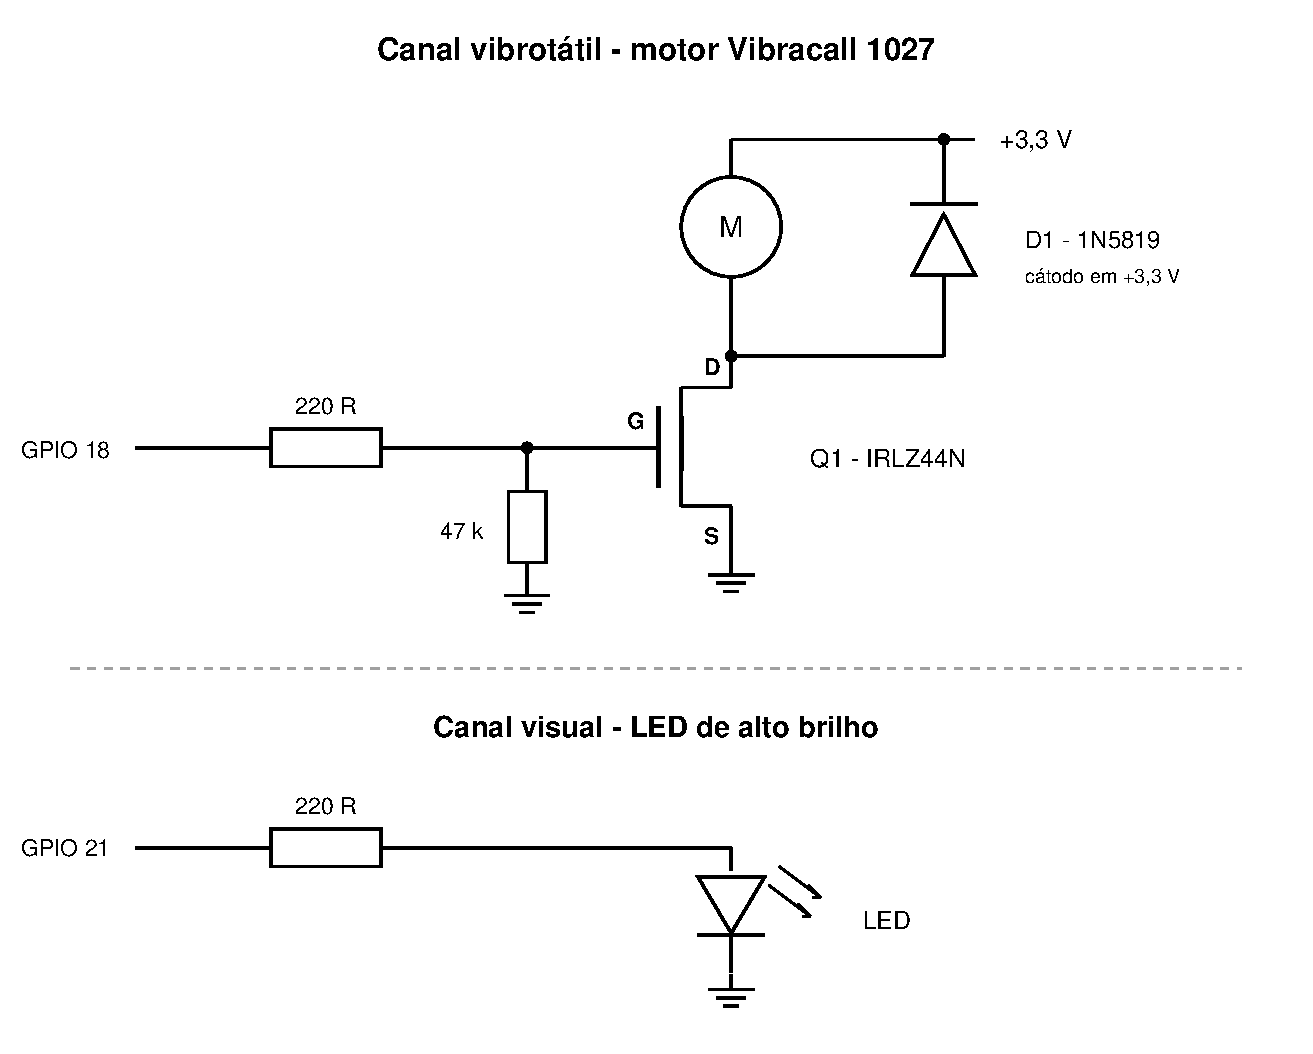
\includegraphics[width=0.90\linewidth,keepaspectratio]{Imagens/Diagramas/circuito_canais_saida.pdf}
\caption{Esquema elétrico dos canais de acionamento vibrotátil e visual}
\label{fig:esquematico_canais_saida}
\legend{Fonte: Elaboração própria (2026).}
\end{figure}

\subsection{Seleção do Transistor MOSFET}
\markright{Metodologia}
\label{sec:selecao_mosfet}


Para o chaveamento do motor vibrotátil foi selecionado o MOSFET IRLZ44N de canal N. O componente é classificado como dispositivo de nível lógico, embora as especificações de resistência de condução do fabricante sejam fornecidas para tensões de gate superiores a 3,3~V \cite{infineonirlz44n}. Por esse motivo, sua utilização foi submetida à avaliação funcional nas condições de corrente do protótipo, sem se assumir saturação plena do transistor na tensão lógica empregada.

O componente foi empregado em configuração \textit{low-side}, na qual o terminal \textit{source} é conectado ao GND do circuito e o terminal \textit{drain} é conectado ao terminal de retorno do motor. O terminal positivo do atuador permanece conectado ao barramento de alimentação.

Essa configuração permite que o sinal PWM gerado pelo ESP32 controle a condução do transistor sem que a corrente necessária ao motor seja fornecida diretamente pelo pino GPIO.

Na configuração final do protótipo foi utilizado um MOSFET IRLZ44N para o canal de acionamento vibrotátil.

\subsection{Resistor de \textit{Gate}}
\markright{Metodologia}
\label{sec:resistor_gate}

Foi utilizado um resistor de 220~$\Omega$ em série entre a saída GPIO do ESP32 responsável pelo controle vibrotátil e o terminal \textit{gate} do MOSFET.

A função desse resistor é limitar as correntes transitórias associadas à carga e descarga da capacitância de entrada do transistor e auxiliar no amortecimento de oscilações durante as transições de chaveamento.

O valor de 220~$\Omega$ foi adotado como compromisso entre a limitação dos transitórios provenientes do GPIO e a manutenção de uma velocidade de chaveamento compatível com o controle PWM empregado no protótipo.

\subsection{Resistor \textit{Pull-Down}}
\markright{Metodologia}
\label{sec:pull_down}


Foi utilizado um resistor \textit{pull-down} de 47~k$\Omega$ conectado entre o terminal \textit{gate} do MOSFET e o GND.

Esse componente mantém o potencial do \textit{gate} próximo de zero quando o pino do microcontrolador se encontra em alta impedância, como pode ocorrer durante a inicialização ou reinicialização do ESP32.

Dessa forma, reduz-se a possibilidade de acionamento involuntário do motor decorrente de um estado elétrico indefinido no terminal de controle do transistor.

O valor de 47~k$\Omega$ foi utilizado por oferecer uma referência definida para o \textit{gate} com baixa corrente estática no circuito de polarização.

\subsection{Proteção contra Transitórios Indutivos}
\markright{Metodologia}
\label{sec:protecao_flyback}


Por apresentar comportamento indutivo, o motor vibrotátil armazena energia durante seu acionamento. Quando a condução do MOSFET é interrompida, a corrente associada à indutância tende a permanecer circulando, podendo produzir transitórios de tensão no estágio de chaveamento.

Para fornecer um caminho de recirculação dessa corrente durante o desligamento, foi utilizado um diodo Schottky 1N5819 conectado em paralelo com o motor e polarizado reversamente durante a operação normal \cite{vishay1n5819}.

O cátodo do diodo foi conectado ao terminal positivo do motor, enquanto o ânodo foi conectado ao terminal associado ao \textit{drain} do MOSFET.

A influência desse elemento de proteção foi posteriormente analisada por meio das simulações elétricas descritas na Seção~\ref{sec:simulacao_flyback}.

\subsection{Estratégia de Alimentação}
\markright{Metodologia}
\label{sec:estrategia_alimentacao}

A estratégia de alimentação do protótipo foi desenvolvida em duas etapas.

Durante a fase inicial de montagem e validação em bancada, o ESP32 foi alimentado por sua interface USB, enquanto o estágio destinado ao motor vibrotátil utilizava uma fonte externa dedicada. Essa configuração facilitou os procedimentos de depuração e permitiu avaliar separadamente os módulos do sistema.

Após a validação funcional da cadeia de controle, foi implementada uma solução de alimentação embarcada com o objetivo de eliminar as conexões físicas entre a estrutura vestível e fontes externas durante a operação.

Para essa configuração foram utilizadas duas células recarregáveis de íons de lítio de 3,7~V associadas em série, formando um conjunto 2S. As células foram associadas a um módulo BMS compatível, destinado à proteção do conjunto.

Como a tensão fornecida pelas baterias é superior à tensão utilizada pelo circuito embarcado, foi empregado um conversor DC--DC baseado no MP1584EN.

O módulo utilizado na montagem é apresentado na Figura~\ref{fig:modulo_mp1584en}. Seu ajuste foi realizado antes da conexão ao restante do circuito, de forma a evitar a aplicação de uma tensão superior à prevista no barramento do sistema embarcado.

\begin{figure}[!htbp]
\centering
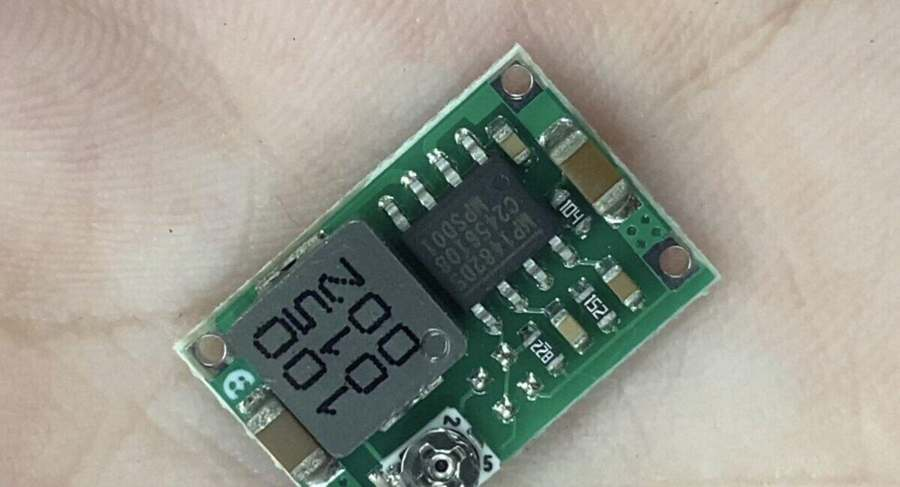
\includegraphics[
width=0.58\linewidth,
keepaspectratio
]{Imagens/Fotos/modulo_mp1584en.jpg}
\caption{Módulo conversor DC--DC utilizado para ajuste da alimentação do circuito embarcado}
\label{fig:modulo_mp1584en}
\legend{Fonte: Elaboração própria (2026).}
\end{figure}


Antes da conexão ao circuito, a saída do conversor foi ajustada com auxílio de multímetro para aproximadamente 3,3~V. Somente após a verificação da tensão de saída o estágio foi conectado ao ESP32 e aos demais elementos da unidade vestível.

Durante os ensaios de integração, a tensão foi monitorada diretamente no barramento de alimentação do microcontrolador enquanto a interface Wi-Fi permanecia ativa. Esse procedimento permitiu verificar o comportamento da alimentação sob uma condição representativa de operação.

O barramento regulado fornece energia ao ESP32 e ao estágio associado ao atuador vibrotátil. Todos os elementos do sistema embarcado compartilham a mesma referência de GND.

A montagem final não utilizou capacitores adicionais de desacoplamento nem fusível resetável PTC. Esses componentes, considerados em etapas preliminares de projeto, não integram a configuração física validada.

A corrente necessária ao motor não é fornecida diretamente pelo GPIO. O pino do ESP32 fornece apenas o sinal PWM aplicado ao \textit{gate} do MOSFET, enquanto a corrente do atuador é proveniente do barramento de alimentação.

Com essa configuração, a unidade vestível passou a operar utilizando alimentação própria, sem necessidade de conexão USB ou de uma fonte externa durante a utilização normal. A comunicação com o computador permanece realizada exclusivamente por Wi-Fi.

O arranjo de alimentação embarcada e sua distribuição funcional são apresentados na Figura~\ref{fig:diagrama_alimentacao_embarcada}. O diagrama representa a organização dos módulos, não o detalhamento dos terminais específicos do BMS.

\begin{figure}[!htbp]
\centering
\resizebox{0.98\linewidth}{!}{\begin{tikzpicture}[
 >=Latex,node distance=5mm and 6mm,
 bloco/.style={draw,rounded corners=3pt,align=center,text width=29mm,minimum height=14mm,font=\small,fill=black!4},
 linha/.style={-Latex,thick}
]
\node[bloco] (bat) {Duas células\\18650 (2S)};
\node[bloco,right=of bat] (bms) {Proteção\\BMS 2S};
\node[bloco,right=of bms] (dc) {Conversor\\MP1584EN};
\node[bloco,right=of dc] (barr) {Barramento\\$+3{,}3$ V / GND};
\draw[linha] (bat) -- (bms);
\draw[linha] (bms) -- (dc);
\draw[linha] (dc) -- (barr);
\node[bloco,below=14mm of barr] (esp) {ESP32-WROOM-32\\alimentação};
\node[bloco,left=of esp] (motor) {Estágio MOSFET\\e motor};
\node[bloco,left=of motor] (led) {LED e resistor\\limitador};
\coordinate (ramo) at ($(barr.south)+(0,-0.35)$);
\draw (barr.south) -- (ramo);
\draw[linha] (ramo) -- (esp.north);
\draw[linha] (ramo) -| (motor.north);
\draw[linha] (ramo) -| (led.north);
\node[font=\scriptsize,below=6mm of motor,align=center] {Os três ramos compartilham\\a referência de GND.};
\end{tikzpicture}
}
\caption{Diagrama funcional do sistema de alimentação embarcada}
\label{fig:diagrama_alimentacao_embarcada}
\legend{Fonte: Elaboração própria (2026).}
\end{figure}


\section{Invólucro e Organização Física do Protótipo}
\markright{Metodologia}
\label{sec:involucro_prototipo}

Após a validação dos módulos eletrônicos em bancada, a montagem foi consolidada em uma placa perfurada, reduzindo o volume ocupado pelas interligações e permitindo acomodar o conjunto em uma estrutura portátil. A Figura~\ref{fig:pci_prototipo} registra as duas faces da placa utilizada no protótipo. Na vista frontal observam-se o ESP32 e os componentes do estágio eletrônico, enquanto a vista posterior evidencia as conexões soldadas responsáveis pela interligação do circuito.

\begin{figure}[!htbp]
\centering
\begin{minipage}[t]{0.47\textwidth}
\centering
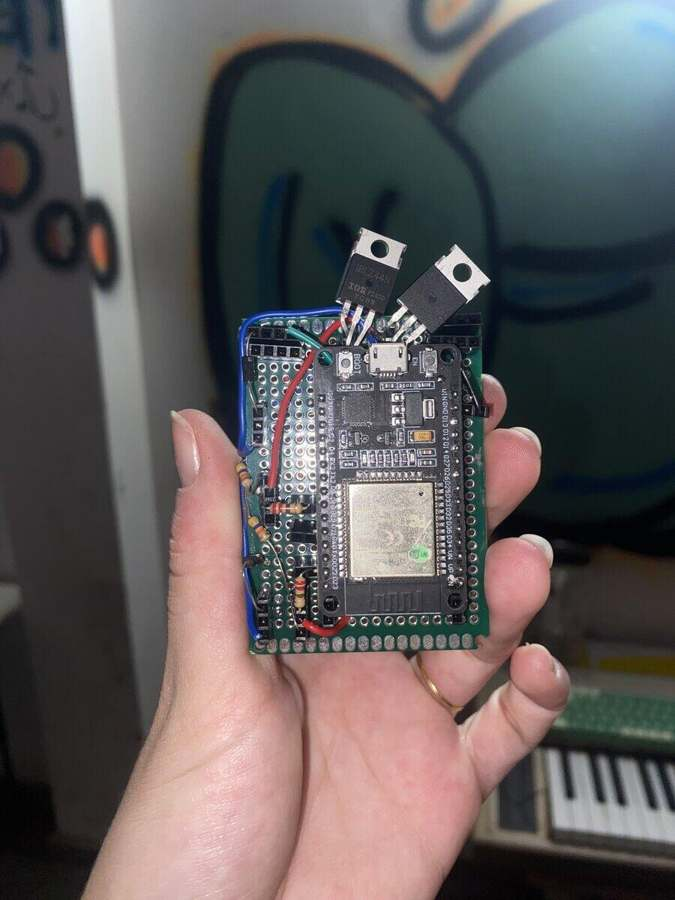
\includegraphics[width=\linewidth]{Imagens/Fotos/pci_frente.jpg}
\end{minipage}
\hfill
\begin{minipage}[t]{0.47\textwidth}
\centering
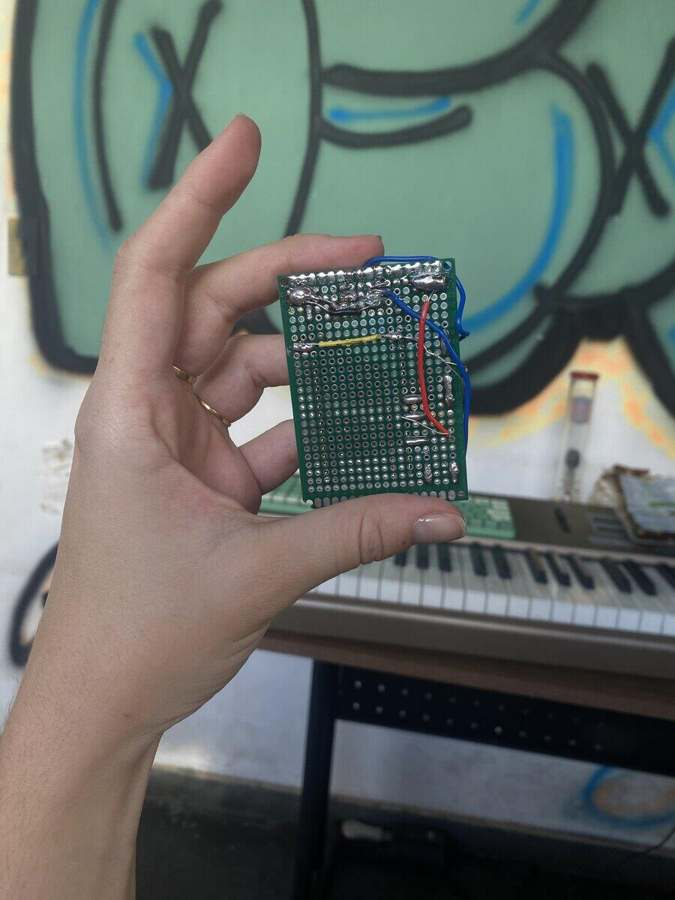
\includegraphics[width=\linewidth]{Imagens/Fotos/pci_verso.jpg}
\end{minipage}
\caption{Montagem do circuito em placa perfurada: vista frontal, à esquerda, e vista posterior, à direita}
\label{fig:pci_prototipo}
\legend{Fonte: Elaboração própria (2026).}
\end{figure}

Com o objetivo de proteger a eletrônica e facilitar sua fixação ao corpo, foi desenvolvido um invólucro específico para a unidade embarcada. O modelo foi dividido em duas peças independentes, constituídas por um corpo principal e uma tampa. Essa separação permitiu manter acesso ao circuito durante as etapas de montagem, depuração e manutenção.

O desenvolvimento do modelo digital contou com apoio do ambiente Cursor \cite{cursor2026}, utilizado como ferramenta auxiliar durante a elaboração e o ajuste da geometria. O uso da ferramenta teve caráter de apoio ao processo de modelagem: as dimensões, a adequação física e as decisões relacionadas à integração dos componentes foram verificadas a partir da montagem real do protótipo.

A geometria final foi exportada em formato STL. O arquivo \texttt{caixa\_corpo.stl} corresponde ao corpo principal do invólucro, enquanto \texttt{caixa\_tampa.stl} corresponde à tampa.

Os arquivos foram preservados como parte do material de reprodução do projeto, permitindo que o invólucro seja fabricado novamente por impressão 3D ou utilizado como ponto de partida para modificações futuras.

A Figura~\ref{fig:modelos_inv_3d} apresenta uma visualização tridimensional dos arquivos STL utilizados no invólucro, com o corpo principal à esquerda e a tampa à direita.

\begin{figure}[!htbp]
\centering
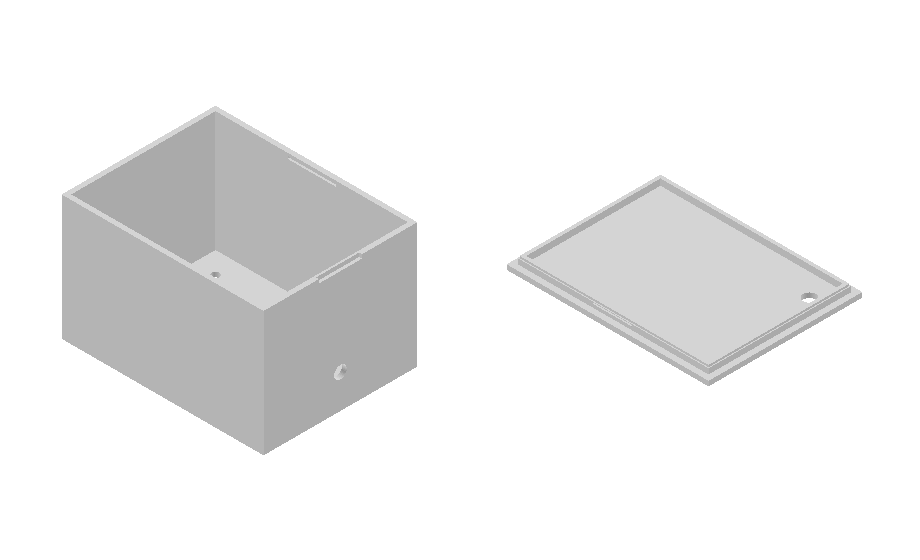
\includegraphics[width=0.95\linewidth,keepaspectratio]{Imagens/Diagramas/modelos_involucro_3d.png}
\caption{Modelos tridimensionais do corpo principal e da tampa do invólucro, renderizados a partir dos arquivos STL do protótipo}
\label{fig:modelos_inv_3d}
\legend{Fonte: Elaboração própria (2026).}
\end{figure}

A Figura~\ref{fig:caixa_motor_led} apresenta detalhes da integração mecânica dos elementos de feedback. Na vista externa, o LED permanece aparente na tampa da caixa, permitindo a observação do canal visual. Na base destinada ao contato com o braço, o motor vibrotátil foi fixado de forma a favorecer a transmissão do estímulo mecânico à região de uso.

\begin{figure}[!htbp]
\centering
\begin{minipage}[t]{0.47\textwidth}
\centering
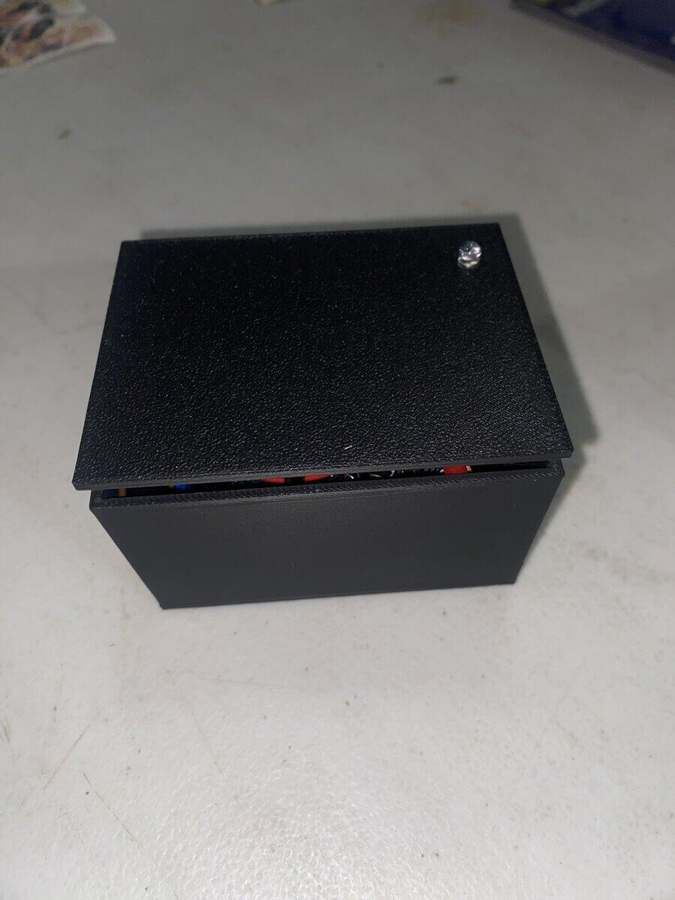
\includegraphics[width=\linewidth]{Imagens/Fotos/caixa_led.jpg}
\end{minipage}
\hfill
\begin{minipage}[t]{0.47\textwidth}
\centering
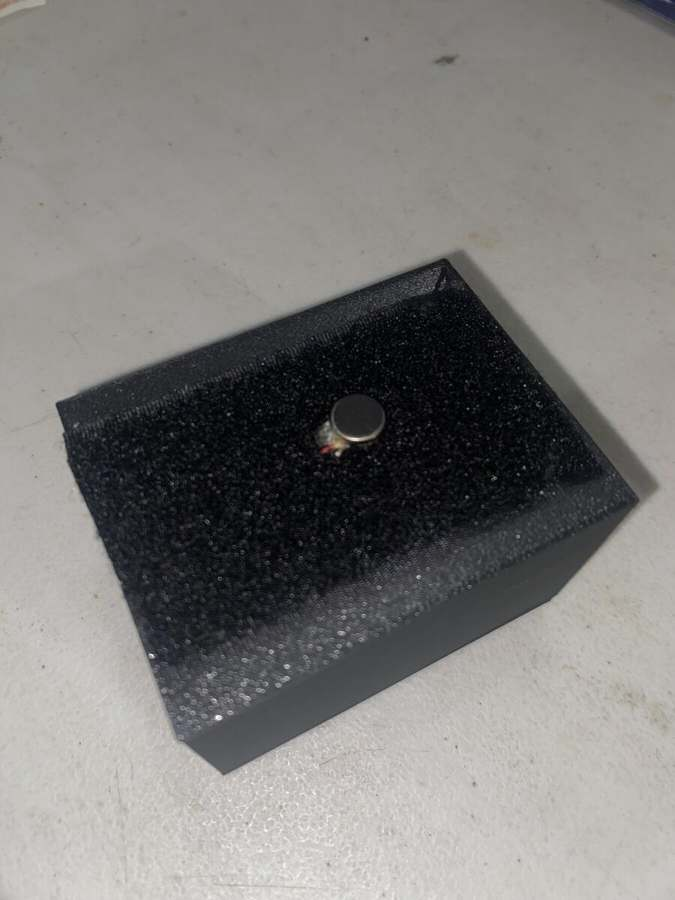
\includegraphics[width=\linewidth]{Imagens/Fotos/fundo_caixa_motor.jpg}
\end{minipage}
\caption{Integração dos elementos de feedback ao invólucro: caixa impressa com o LED aparente, à esquerda, e base com o motor vibrotátil fixado, à direita}
\label{fig:caixa_motor_led}
\legend{Fonte: Elaboração própria (2026).}
\end{figure}

A fixação ao antebraço foi realizada por meio de uma faixa de velcro. A Figura~\ref{fig:elementos_vestiveis} mostra, antes da montagem no usuário, a pulseira e a caixa com o motor posicionado na superfície destinada ao contato com o braço.

\begin{figure}[!htbp]
\centering
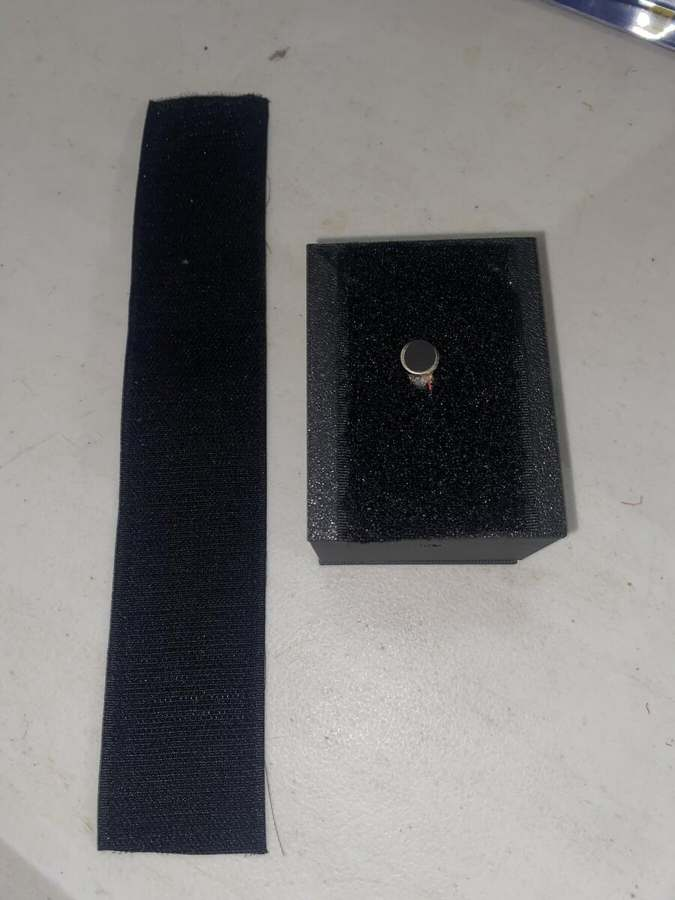
\includegraphics[
width=0.48\linewidth,
keepaspectratio
]{Imagens/Fotos/pulseira_caixa_componentes.jpg}
\caption{Pulseira de velcro e caixa impressa utilizadas na configuração vestível do protótipo}
\label{fig:elementos_vestiveis}
\legend{Fonte: Elaboração própria (2026).}
\end{figure}

A configuração final montada no antebraço é apresentada na Figura~\ref{fig:prototipo_final_vestivel}. As duas vistas registram a disposição da caixa sobre a pulseira e a posição do LED na face superior. A solução deve ser entendida como uma implementação experimental para validação da arquitetura. Não foram conduzidos ensaios formais de ergonomia, conforto prolongado, distribuição de massa, pressão de contato ou posicionamento ótimo do atuador.

\begin{figure}[!htbp]
\centering
\begin{minipage}[t]{0.47\textwidth}
\centering
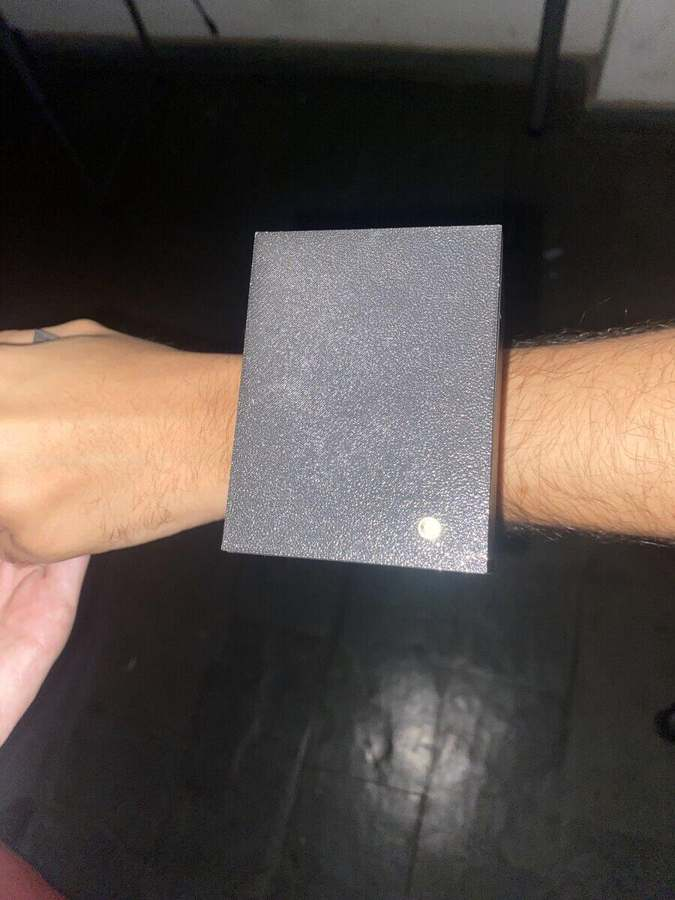
\includegraphics[width=\linewidth]{Imagens/Fotos/prototipo_final_superior.jpg}
\end{minipage}
\hfill
\begin{minipage}[t]{0.47\textwidth}
\centering
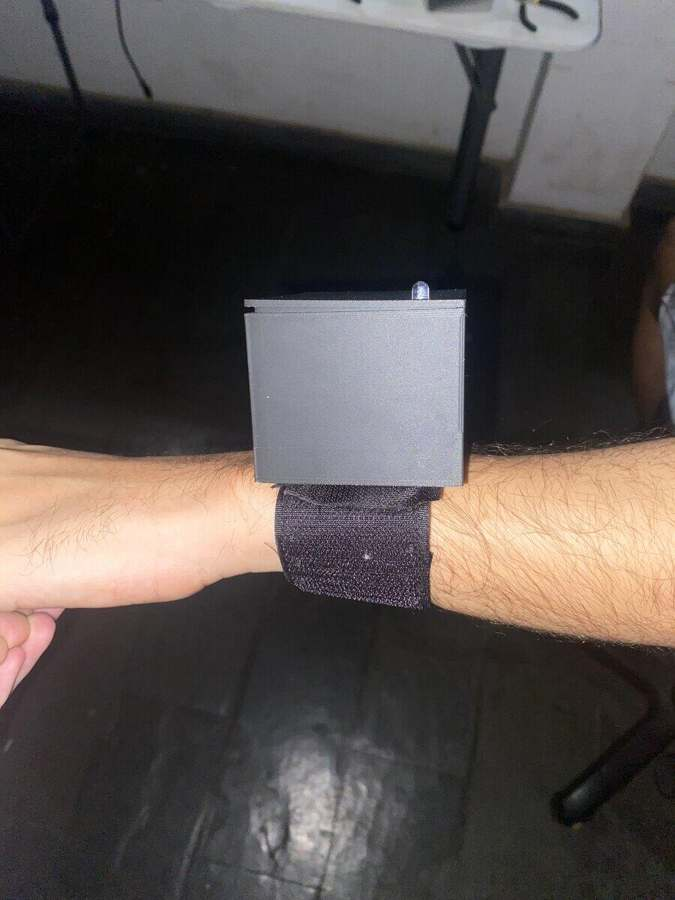
\includegraphics[width=\linewidth]{Imagens/Fotos/prototipo_final_lateral.jpg}
\end{minipage}
\caption{Protótipo final em configuração vestível: vista superior, à esquerda, e vista lateral, à direita}
\label{fig:prototipo_final_vestivel}
\legend{Fonte: Elaboração própria (2026).}
\end{figure}

A documentação pública associada ao trabalho reúne os modelos tridimensionais, instruções de montagem, organização do hardware e arquivos de software necessários à reprodução do sistema.


\section{Simulação do Circuito Eletrônico}
\markright{Metodologia}
\label{sec:simulacao_circuito}

Antes da integração física completa do circuito de acionamento, foram realizadas simulações elétricas utilizando o software LTspice.

Essa etapa teve como objetivo analisar previamente o comportamento do estágio eletrônico responsável pelo acionamento do motor vibrotátil em condições representativas de operação.

As simulações foram realizadas considerando um único canal de acionamento, correspondente à topologia posteriormente implementada no protótipo físico.

Foram investigados dois aspectos principais: a atuação do diodo de \textit{flyback} durante o desligamento da carga indutiva e o comportamento do circuito para diferentes valores de \textit{duty cycle} do sinal PWM.

Os resultados obtidos a partir dessas simulações são apresentados e discutidos no Capítulo 5.

\subsection{Modelo Elétrico Utilizado}
\markright{Metodologia}
\label{sec:modelo_eletrico_simulacao}

O modelo utilizado no LTspice representa o estágio eletrônico empregado para o acionamento do motor vibrotátil.

O circuito simulado é constituído por uma fonte de alimentação de 3,3~V, um modelo simplificado do motor vibrotátil baseado em uma associação resistiva-indutiva, um transistor MOSFET de canal N em configuração \textit{low-side}, resistor de gate, resistor \textit{pull-down} e diodo de \textit{flyback}.

A representação resistiva-indutiva foi utilizada como aproximação do comportamento elétrico de um motor de corrente contínua durante as análises transitórias.

O modelo não busca reproduzir integralmente o comportamento eletromecânico do Vibracall 1027, mas possibilitar a avaliação qualitativa dos fenômenos elétricos associados ao chaveamento de uma carga indutiva.

O MOSFET foi comandado por um sinal pulsado representativo do PWM produzido pelo ESP32.

Durante as diferentes análises, foram mantidas as características gerais da topologia, alterando-se apenas os parâmetros necessários para cada cenário de simulação.


A Figura~\ref{fig:simulacao_circuito_base} apresenta uma configuração exploratória do circuito-base utilizado nas análises. A imagem inclui componentes auxiliares de simulação, como capacitores e resistência de alimentação, que não foram incorporados à montagem final do protótipo.

\begin{figure}[!htbp]
\centering
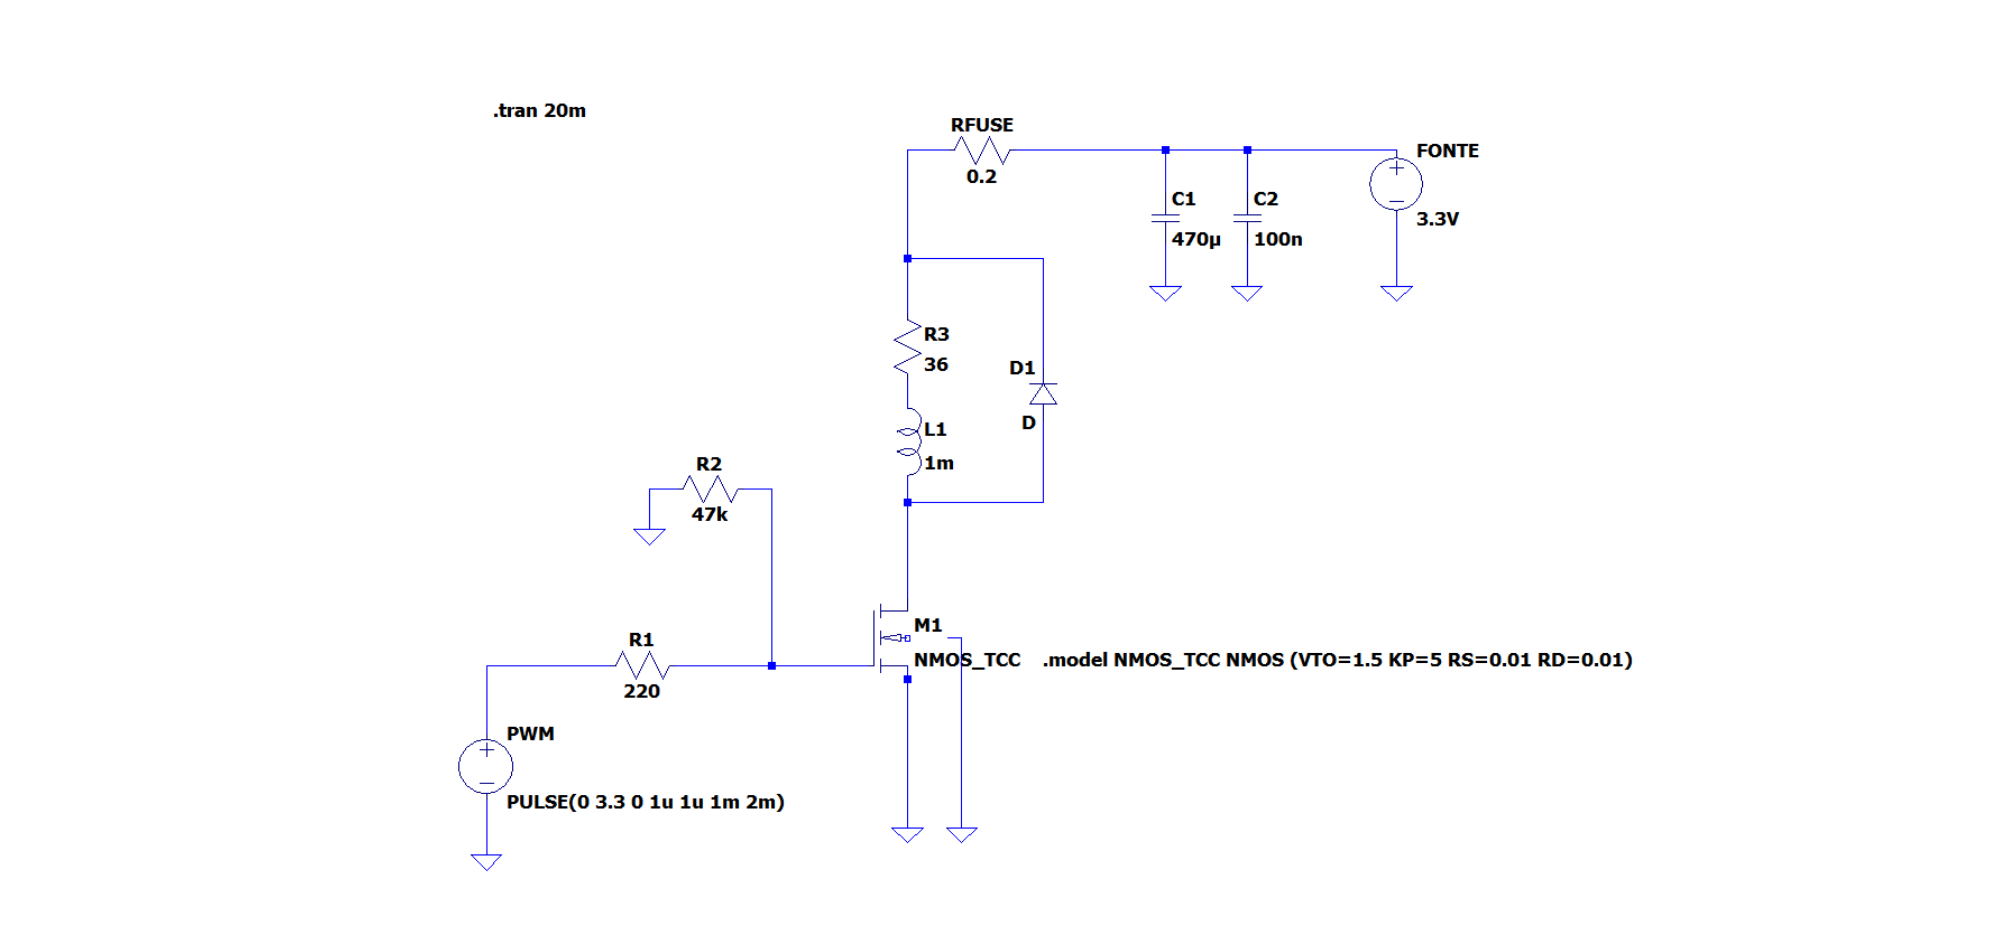
\includegraphics[
width=0.52\linewidth,
trim=240bp 50bp 235bp 35bp,
clip,
keepaspectratio
]{Metodologia/simulacao_circuito_base.png}
\caption{Circuito-base exploratório do acionamento vibrotátil modelado no LTspice}
\label{fig:simulacao_circuito_base}
\legend{Fonte: Elaboração própria (2026).}
\end{figure}

\subsection{Simulação da Proteção por Diodo de \textit{Flyback}}
\markright{Metodologia}
\label{sec:simulacao_flyback}

A influência do diodo de \textit{flyback} foi analisada por meio da comparação entre duas configurações do mesmo estágio eletrônico de acionamento.

Na primeira configuração, foi mantido o diodo Schottky 1N5819 conectado em paralelo com a carga indutiva e polarizado reversamente durante a operação normal.

Na segunda configuração, o componente foi removido do circuito.

Para ambas as condições foram mantidos os demais parâmetros da simulação, permitindo comparar o comportamento transitório produzido durante a interrupção da condução do MOSFET.

A análise foi direcionada principalmente ao comportamento da tensão no estágio de chaveamento e da corrente associada à carga indutiva após a interrupção da condução.

Essa comparação foi utilizada para verificar qualitativamente a função do caminho de recirculação de corrente proporcionado pelo diodo.

As formas de onda obtidas nas configurações com e sem o diodo de \textit{flyback} são apresentadas e discutidas no Capítulo 5.

\subsection{Simulação do Controle PWM}
\markright{Metodologia}
\label{sec:simulacao_pwm}

Para avaliar o comportamento do estágio eletrônico diante de diferentes níveis de comando PWM, foram realizadas simulações mantendo constante a frequência de chaveamento e variando o \textit{duty cycle} do sinal aplicado ao MOSFET.

Foram considerados três níveis de operação:

20\%, 50\% e 80\%.

Para cada condição foram registradas as formas de onda associadas ao acionamento da carga equivalente.

A utilização de diferentes razões cíclicas permitiu comparar o comportamento elétrico do modelo diante de condições de acionamento reduzido, intermediário e elevado.

Essa etapa teve como objetivo verificar qualitativamente se a variação do \textit{duty cycle} produz alterações correspondentes na energia média fornecida à carga equivalente.

Os resultados obtidos para os três níveis de \textit{duty cycle} são apresentados e comparados no Capítulo 5.

\section{Comunicação entre Computador e ESP32}
\markright{Metodologia}
\label{sec:comunicacao_udp}

A comunicação entre o computador responsável pelo processamento das mensagens MIDI e o microcontrolador ESP32 foi implementada por meio do protocolo UDP sobre uma rede Wi-Fi local.

O software desenvolvido em Python é responsável por gerar e transmitir os comandos de controle, enquanto o ESP32 permanece associado à mesma rede e monitora uma porta UDP previamente configurada para receber as mensagens enviadas pelo computador.

Após a recepção de cada comando, o microcontrolador realiza sua interpretação e atualiza as saídas PWM utilizadas pelo sistema.

A utilização do protocolo UDP foi adotada devido à simplicidade da troca de datagramas entre os módulos e à ausência da necessidade de estabelecimento prévio de uma conexão entre o computador e o microcontrolador.

O UDP fornece um mecanismo mínimo de transporte de datagramas e não incorpora mecanismos próprios de confirmação de entrega ou retransmissão \cite{postel1980udp}.

Por esse motivo, foi incluído na metodologia um procedimento específico para avaliar o comportamento da comunicação durante transmissões sucessivas.

\subsection{Formato das Mensagens de Comunicação}
\markright{Metodologia}
\label{sec:formato_mensagens_udp}

Durante a operação normal do sistema, os comandos enviados pelo software em Python informam ao ESP32 o estado de acionamento e, quando aplicável, o valor PWM correspondente.

Para o acionamento das saídas foi utilizado o formato:

\begin{center}
\texttt{ON,valor\_pwm}
\end{center}

em que \texttt{valor\_pwm} representa o nível de controle calculado a partir do parâmetro \textit{velocity} da mensagem MIDI.

Para interromper o acionamento foi utilizado o comando:

\begin{center}
\texttt{OFF}
\end{center}

Após a interpretação da mensagem, o ESP32 aplica o valor PWM recebido ao canal vibrotátil e ao canal visual.

Na configuração implementada, o GPIO 18 controla o estágio de acionamento do motor Vibracall 1027, enquanto o GPIO 21 controla o LED de alto brilho.

Para os ensaios específicos de estabilidade da comunicação, o formato das mensagens foi ampliado com a inclusão de um identificador sequencial de pacote, permitindo comparar os registros de transmissão e recepção.

Nesse caso, os pacotes de teste foram enviados no formato:

\begin{center}
\texttt{ON,id,pwm}
\end{center}

Nesse formato, \texttt{ON} identifica o comando de acionamento, \texttt{id} corresponde ao número sequencial do pacote e \texttt{pwm} representa o valor de controle transmitido ao ESP32.

\subsection{Procedimento de Teste da Comunicação UDP}
\markright{Metodologia}
\label{sec:teste_estabilidade_udp}

Com o objetivo de avaliar o comportamento da comunicação durante transmissões sucessivas, foi implementado um ensaio baseado no envio automatizado de uma sequência de pacotes UDP entre o computador e o ESP32.

O procedimento foi configurado para transmitir 100 pacotes de teste numerados sequencialmente.

Antes do início da sequência utilizada para análise, foi transmitida uma mensagem identificada como \texttt{PING}, empregada como etapa preliminar de inicialização da comunicação.

Os pacotes foram enviados com intervalo aproximado de 50~ms entre transmissões consecutivas.

No computador, o software em Python registrou o identificador de cada pacote, o comando transmitido e o instante relativo de envio.

No ESP32, o monitor serial foi utilizado para registrar os identificadores dos pacotes recebidos e os respectivos instantes relativos de recepção, obtidos a partir da função \texttt{millis()}.

Após a execução do ensaio, os registros produzidos nos dois módulos foram comparados quanto à quantidade de pacotes transmitidos e recebidos, à correspondência entre os identificadores e à regularidade temporal da sequência.

O teste foi utilizado como procedimento de avaliação da estabilidade da comunicação entre os módulos.

Os registros experimentais, a quantidade de pacotes efetivamente recebidos e a análise dos dados temporais são apresentados no Capítulo 5.

\section{Implementação Computacional}
\markright{Metodologia}
\label{sec:implementacao_computacional}

A implementação em Python concentrou no computador a aquisição e o processamento MIDI, o cálculo PWM, a interface gráfica e a preparação dos comandos. O ESP32 recebeu esses comandos para controlar as saídas físicas, permitindo ensaiar separadamente o software e o módulo embarcado.

\subsection{Processamento Computacional e Software}
\markright{Metodologia}
\label{sec:processamento_software}

O software em Python estabelece a ligação entre o controlador MIDI e o módulo embarcado. As bibliotecas \textit{mido} e \textit{python-rtmidi} são utilizadas para acessar a interface MIDI conectada ao computador. A comunicação UDP é implementada por meio de \textit{sockets}.

Durante a execução, o programa monitora as mensagens do MPD218, identifica eventos de acionamento e liberação, obtém a nota e a \textit{velocity} e aplica a função de mapeamento definida para o sistema. O valor calculado atualiza a interface gráfica e compõe o comando transmitido ao ESP32. No encerramento do evento, o software envia o comando de desligamento.

A interface gráfica apresenta os 16 \textit{pads} do controlador e exibe o \textit{pad} acionado, a nota MIDI, a \textit{velocity} e o valor PWM calculado. Essa visualização é um recurso de monitoramento e demonstração no computador; o LED incorporado à unidade vestível constitui a saída visual física destinada ao usuário.

A Figura~\ref{fig:fluxograma_algoritmo} representa o fluxo de processamento dos eventos MIDI, incluindo o filtro temporal, o cálculo do PWM e os comandos transmitidos ao ESP32. A operação descrita corresponde ao programa principal de controle, distinto do mapeamento específico empregado no ensaio de queda.

\begin{figure}[!htbp]
\centering
\resizebox{0.95\linewidth}{!}{\begin{tikzpicture}[
 >=Latex,node distance=6mm and 7mm,
 caixa/.style={draw,rounded corners=2pt,align=center,font=\footnotesize,minimum height=8mm,text width=35mm,fill=black!3},
 decisao/.style={diamond,aspect=2.15,draw,align=center,font=\footnotesize,inner sep=1pt,text width=27mm,fill=black!3},
 seta/.style={-Latex,thick},
 nota/.style={font=\scriptsize,fill=white,inner sep=1pt}
]
\node[caixa] (midi) {Evento MIDI do MPD218};
\node[decisao,below=10mm of midi] (on) {\texttt{note\_on} e \textit{velocity} $>0$?};
\node[decisao,below left=12mm and 20mm of on] (off) {\texttt{note\_off} ou \textit{velocity} $=0$?};
\node[decisao,below right=12mm and 20mm of on] (db) {Intervalo $\geq 0{,}08$ s?};
\node[caixa,below=12mm of off] (sendoff) {Enviar \texttt{OFF} por UDP};
\node[caixa,below=12mm of db] (map) {Calcular PWM proporcional; limitar a 80--255};
\node[caixa,below=7mm of map] (sendon) {Atualizar interface e CSV; enviar \texttt{ON,PWM}};
\node[caixa,below=14mm of sendoff] (zero) {ESP32 aplica PWM 0 ao motor e LED};
\node[caixa,below=7mm of sendon] (motor) {ESP32 aplica PWM aos GPIO 18 e 21};
\draw[seta] (midi) -- (on);
\draw[seta] (on) -| node[nota,pos=.22] {Não} (off);
\draw[seta] (on) -| node[nota,pos=.22] {Sim} (db);
\draw[seta] (off) -- node[nota] {Sim} (sendoff);
\draw[seta] (db) -- node[nota] {Sim} (map);
\draw[seta] (sendoff) -- (zero);
\draw[seta] (map) -- (sendon);
\draw[seta] (sendon) -- (motor);
\node[nota,below=1mm of zero] {Ambas as saídas desligadas};
\node[nota,below=1mm of motor] {Resposta vibrotátil e visual};
\draw[seta] (off.west) -- ++(-9mm,0) node[nota,anchor=east] {Não: ignorar};
\draw[seta] (db.east) -- ++(9mm,0) node[nota,anchor=west] {Não: ignorar};
\end{tikzpicture}
}
\caption{Fluxograma do processamento de eventos MIDI e geração dos comandos de atuação}
\label{fig:fluxograma_algoritmo}
\legend{Fonte: Elaboração própria (2026).}
\end{figure}

\subsection{Aquisição e Tratamento dos Eventos MIDI}
\markright{Metodologia}
\label{sec:aquisicao_midi}

A aquisição das mensagens MIDI foi realizada a partir do controlador Akai MPD218 conectado ao computador por meio de interface USB (Akai Professional, 2015).

No ambiente Python, foram utilizadas as bibliotecas \textit{mido} e \textit{python-rtmidi} para acesso à interface MIDI e leitura das mensagens produzidas durante a interação com os pads.

O software identifica os eventos associados ao acionamento e ao encerramento da interação.

Para os eventos válidos de acionamento, são extraídos o número da nota MIDI e o valor de \textit{velocity}.

O número da nota é utilizado na interface gráfica para identificar o pad correspondente, enquanto o valor de \textit{velocity} é utilizado como variável de entrada para o cálculo do nível de controle.

O número da nota MIDI não é utilizado para selecionar individualmente o atuador vibrotátil.

Na estratégia implementada, o valor PWM calculado a partir da \textit{velocity} é utilizado como referência tanto para o canal vibrotátil quanto para o canal visual.

Os eventos associados ao encerramento do acionamento são utilizados para gerar o comando responsável pela interrupção das duas saídas.

\subsection{Tratamento Temporal dos Eventos MIDI}
\markright{Metodologia}
\label{sec:debounce_midi}

Durante os testes iniciais de aquisição MIDI, foram identificados eventos consecutivos registrados em intervalos temporais reduzidos durante a interação com os pads do controlador.

Com o objetivo de evitar que eventos sucessivos dentro de um intervalo mínimo fossem interpretados como novos acionamentos válidos, foi implementado no software um mecanismo de filtragem temporal.

A estratégia adotada consiste em comparar o instante de cada novo evento com o instante do último evento aceito pelo sistema. Um novo acionamento somente é processado quando o intervalo transcorrido é superior ao limite definido para o filtro.

Durante o desenvolvimento, foi utilizado um intervalo de aproximadamente 80~ms.

A condição de filtragem pode ser representada por:

\begin{equation}
t_{\mathrm{atual}} - t_{\mathrm{ultimo}} < t_{\mathrm{filtro}},
\label{eq:filtro_temporal_midi}
\end{equation}

em que $t_{\mathrm{atual}}$ representa o instante do evento recebido, $t_{\mathrm{ultimo}}$ o instante do último evento considerado válido e $t_{\mathrm{filtro}}$ o intervalo mínimo adotado para a filtragem temporal.

Quando a condição apresentada é satisfeita, o novo evento é desconsiderado para fins de acionamento. Caso contrário, ele é processado normalmente e seu instante passa a ser utilizado como nova referência temporal.

A implementação dessa lógica foi realizada utilizando recursos de medição de tempo disponíveis no ambiente Python.

\subsection{Registro dos Dados Computacionais}
\markright{Metodologia}
\label{sec:registro_dados_computacionais}

Durante os procedimentos de desenvolvimento e validação, o software foi configurado para registrar informações associadas aos eventos processados.

Os registros foram armazenados em arquivos CSV contendo, conforme o ensaio realizado, informações como número da nota MIDI, valor de \textit{velocity} e valor PWM calculado.

Além dos arquivos estruturados, os terminais utilizados durante a execução do software permitiram acompanhar os comandos transmitidos ao sistema embarcado.

Esses registros foram utilizados posteriormente para analisar o comportamento do algoritmo e elaborar os gráficos apresentados no Capítulo 5.


\section{Estratégia de Controle Multissensorial}
\markright{Metodologia}
\label{sec:estrategia_controle}

A estratégia de controle converte o parâmetro \textit{velocity} do evento MIDI em um comando PWM calculado no computador. O ESP32 aplica o nível recebido ao motor conectado ao estágio MOSFET (GPIO 18) e ao LED (GPIO 21). As saídas compartilham a referência digital, sem pressupor equivalência entre intensidade de vibração, brilho e percepção do usuário.

\subsection{Mapeamento entre \textit{Velocity} MIDI e PWM}
\markright{Metodologia}
\label{sec:mapeamento_velocity_pwm}

O parâmetro \textit{velocity} foi utilizado como variável de entrada para determinar o valor de controle aplicado às modalidades de feedback.

Durante a implementação, foi adotado um mapeamento proporcional entre os valores de \textit{velocity} registrados pelo controlador MIDI e a faixa de PWM definida para o sistema.

O algoritmo implementado considera como referência superior o valor de \textit{velocity} igual a 30. Para valores até esse limite, o comando PWM é calculado proporcionalmente por:

\begin{equation}
P_{\mathrm{PWM}} =
\frac{V_{\mathrm{MIDI}}}{30}
\cdot 255
\end{equation}

em que $V_{\mathrm{MIDI}}$ representa o valor de \textit{velocity} recebido e $P_{\mathrm{PWM}}$ representa o valor PWM calculado.

Após o cálculo, é aplicado um limite inferior de 80 aos eventos válidos de acionamento. Dessa forma, valores calculados abaixo desse limite são ajustados para 80.

Valores de \textit{velocity} superiores à referência utilizada produzem valores calculados acima da faixa PWM disponível e são saturados em 255.

A lógica pode ser representada por:

\begin{equation}
P_{\mathrm{PWM}} =
\min
\left(
255,
\max
\left(
80,
\frac{V_{\mathrm{MIDI}}}{30}\cdot255
\right)
\right)
\end{equation}

para eventos de acionamento com \textit{velocity} maior que zero.

O cálculo é realizado no software em Python antes da transmissão ao ESP32.

Na configuração final, o valor resultante é utilizado como referência simultaneamente para o canal vibrotátil e para o canal visual.

Para análise do comportamento do algoritmo, os pares formados pelos valores de \textit{velocity} e pelos respectivos valores PWM calculados foram registrados durante os ensaios.


\subsection{Intervalo de Operação PWM}
\markright{Metodologia}
\label{sec:intervalo_operacao_pwm}

Para o controle dos atuadores foi utilizada uma faixa de PWM compreendida entre 80 e 255 para os eventos válidos de acionamento.

O valor 255 corresponde ao limite superior utilizado na representação PWM adotada na implementação. Valores calculados acima desse limite são saturados em 255.

O valor inferior de 80 foi adotado durante o desenvolvimento para evitar a utilização de comandos muito reduzidos, associados a uma região de acionamento pouco útil para os motores no protótipo experimental.

Assim, para um evento MIDI válido, o comando produzido pelo software permanece limitado ao intervalo:

\begin{equation}
80 \leq P_{\mathrm{PWM}} \leq 255,
\label{eq:intervalo_pwm}
\end{equation}

em que $P_{\mathrm{PWM}}$ representa o valor de controle posteriormente aplicado pelo ESP32 aos canais vibrotátil e visual.

A definição dessa faixa foi utilizada como parâmetro de implementação do protótipo. Sua adequação é discutida no Capítulo 5 a partir dos ensaios realizados com o sistema.

\subsection{Tratamento dos Comandos de Acionamento}
\markright{Metodologia}
\label{sec:comandos_acionamento}

Os formatos \texttt{ON,valor\_pwm} e \texttt{OFF} estão especificados na Seção~\ref{sec:formato_mensagens_udp}. O software envia o comando de acionamento para eventos válidos do tipo \texttt{note\_on} com \textit{velocity} maior que zero. Eventos \texttt{note\_off} e mensagens \texttt{note\_on} com \textit{velocity} igual a zero são tratados como encerramento da nota \cite{midi1996}.

Ao receber \texttt{ON}, o ESP32 atualiza as saídas PWM associadas ao motor e ao LED. O comando \texttt{OFF} atribui valor zero às duas saídas. Assim, a duração de cada resposta acompanha os eventos de acionamento e liberação enviados pelo controlador.


\section{Procedimentos Experimentais de Validação}
\markright{Metodologia}
\label{sec:procedimentos_experimentais}

Os procedimentos experimentais foram definidos com o objetivo de validar progressivamente os diferentes módulos da arquitetura desenvolvida e, posteriormente, verificar seu funcionamento integrado.

A estratégia adotada foi incremental. Inicialmente foram avaliados os sinais de controle e o estágio eletrônico responsável pelo acionamento do motor vibrotátil. Em seguida, foi realizada a validação física do atuador, da comunicação entre o computador e o ESP32 e da alimentação embarcada.

Após a validação do canal vibrotátil, foi incorporado o LED de alto brilho utilizado como modalidade física de feedback visual.

Por fim, foi avaliada a operação simultânea das duas modalidades de saída durante a interação com o controlador MIDI, utilizando a cadeia completa formada pelo Akai MPD218, software em Python, comunicação UDP sobre Wi-Fi, ESP32, motor vibrotátil e LED.

Essa sequência permitiu identificar e corrigir falhas individualmente antes da integração completa do protótipo e reduzir os riscos associados à energização simultânea dos diferentes módulos.


\subsection{Validação do Estágio de Chaveamento}
\markright{Metodologia}
\label{sec:validacao_chaveamento}


Antes da conexão do motor vibrotátil, foi realizada uma validação preliminar do estágio eletrônico utilizando um LED como carga auxiliar de teste.

O ensaio foi conduzido com uma saída GPIO do ESP32 conectada ao terminal \textit{gate} do MOSFET IRLZ44N por meio do resistor de 220~$\Omega$, mantendo também o resistor \textit{pull-down} previsto no circuito.

Foram aplicados diferentes estados de acionamento com o objetivo de verificar o caminho de controle entre o ESP32, o MOSFET e a carga antes da utilização do motor.

Nessa etapa, o LED foi utilizado exclusivamente como ferramenta de depuração do circuito eletrônico, não correspondendo ainda ao canal visual posteriormente incorporado à arquitetura final.


\subsection{Validação de um Canal Vibrotátil}
\markright{Metodologia}
\label{sec:validacao_um_canal}

Após a verificação inicial do estágio eletrônico, foi realizada a validação física utilizando um motor Vibracall 1027 conectado ao circuito de acionamento.

A montagem foi composta pelo ESP32, transistor MOSFET IRLZ44N, resistor de gate, resistor \textit{pull-down}, diodo de \textit{flyback} e motor vibrotátil.

Inicialmente foram realizados testes de continuidade e medições de tensão nos diferentes pontos do circuito com o objetivo de verificar a propagação do sinal de controle entre o GPIO do ESP32 e o terminal \textit{gate} do MOSFET.

Em seguida, comandos transmitidos por UDP foram utilizados para verificar o acionamento e o desligamento do motor.

Posteriormente, o controlador Akai MPD218 foi utilizado para produzir eventos MIDI com diferentes valores de \textit{velocity}. O software desenvolvido em Python processou esses eventos, calculou os valores PWM correspondentes e transmitiu os comandos ao ESP32.


\subsection{Ensaio com Corpo de Massa Conhecida}
\markright{Metodologia}
\label{sec:ensaio_queda_controlada}

Após a validação funcional do canal vibrotátil, foi realizado um ensaio específico para investigar a correspondência entre uma condição mecânica de entrada controlada, o valor de \textit{velocity} fornecido pelo MPD218 e o comando PWM calculado pelo software.

Antes da definição do procedimento definitivo, foi realizado um ensaio exploratório de carregamento estático sobre um dos pads. Nessa montagem, massas foram acrescentadas progressivamente até a ocorrência de acionamento, conforme ilustrado na Figura~\ref{fig:ensaio_estatico_exploratorio}. Esse procedimento foi utilizado apenas como referência preliminar de sensibilidade do pad. Como o parâmetro \textit{velocity} é determinado pelo comportamento dinâmico do acionamento e não por uma carga estática isolada, o ensaio foi mantido apenas como registro exploratório e não integrou a análise quantitativa principal.

\begin{figure}[!htbp]
\centering
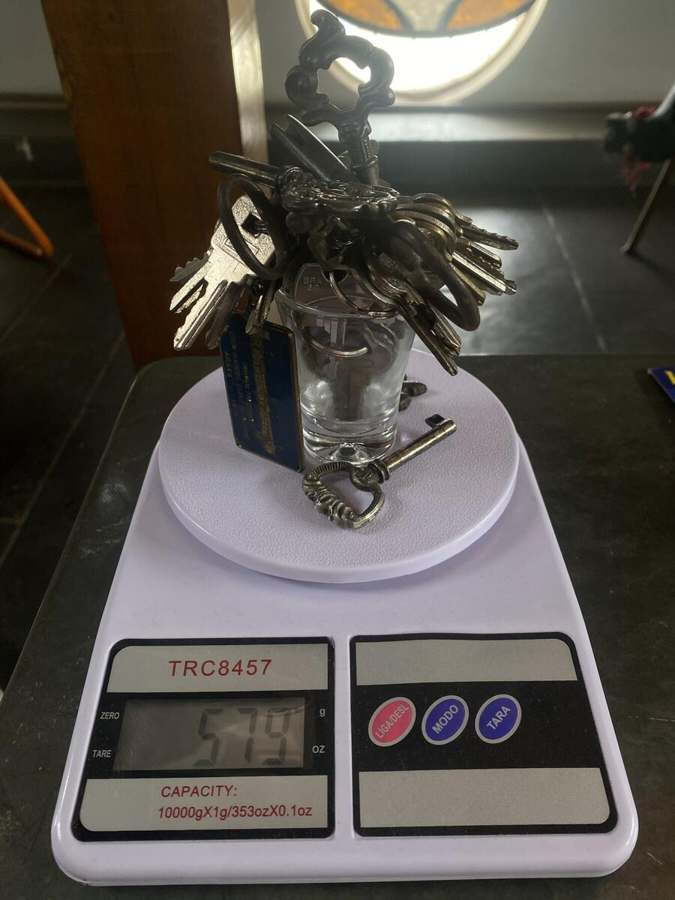
\includegraphics[
width=0.50\linewidth,
keepaspectratio
]{Imagens/Fotos/ensaio_estatico_limiar_pad.jpg}
\caption{Ensaio exploratório de carregamento estático empregado na definição do procedimento experimental}
\label{fig:ensaio_estatico_exploratorio}
\legend{Fonte: Elaboração própria (2026).}
\end{figure}


Foi utilizado um corpo com massa de 39~g, solto sobre o pad 4 do controlador, correspondente à nota MIDI 71. A altura de queda foi medida com régua e variada entre 0,5~cm e 5~cm, nas condições de 0,5; 1; 2; 3; 4 e 5~cm. Para cada altura foram realizadas dez repetições, totalizando 60 quedas independentes. O corpo foi liberado sem impulso adicional, procurando-se manter a região de impacto sobre o mesmo pad.

A Figura~\ref{fig:ensaio_queda_massa} documenta o corpo utilizado e a configuração adotada para controle da altura. A massa foi conferida em balança antes da coleta, e uma régua foi utilizada como referência para posicionar o corpo antes de cada liberação.

\begin{figure}[!htbp]
\centering
\begin{minipage}[t]{0.43\textwidth}
\centering
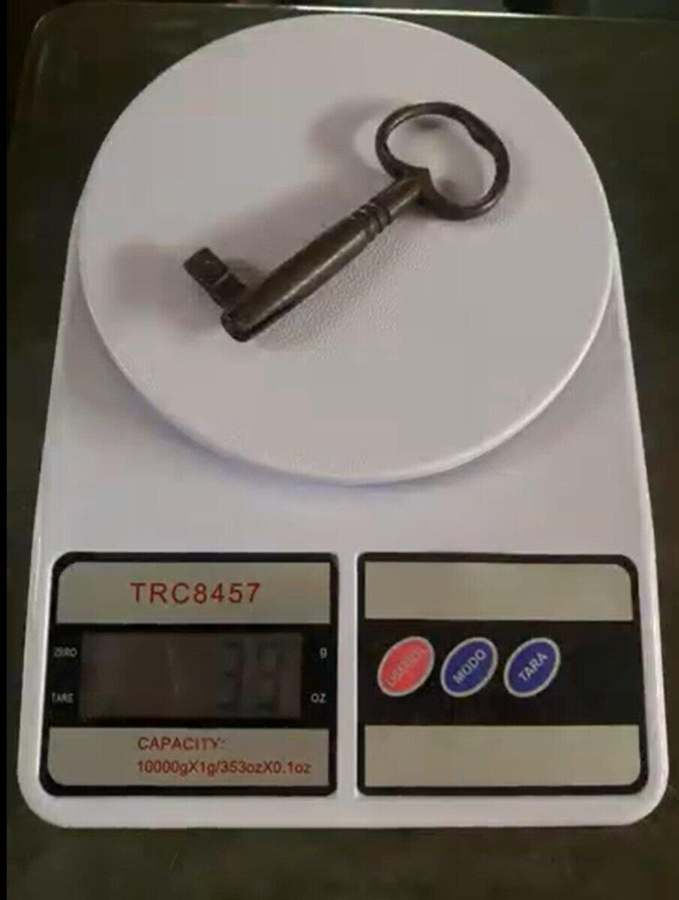
\includegraphics[width=\linewidth]{Imagens/Fotos/massa_39g.jpg}
\end{minipage}
\hfill
\begin{minipage}[t]{0.43\textwidth}
\centering
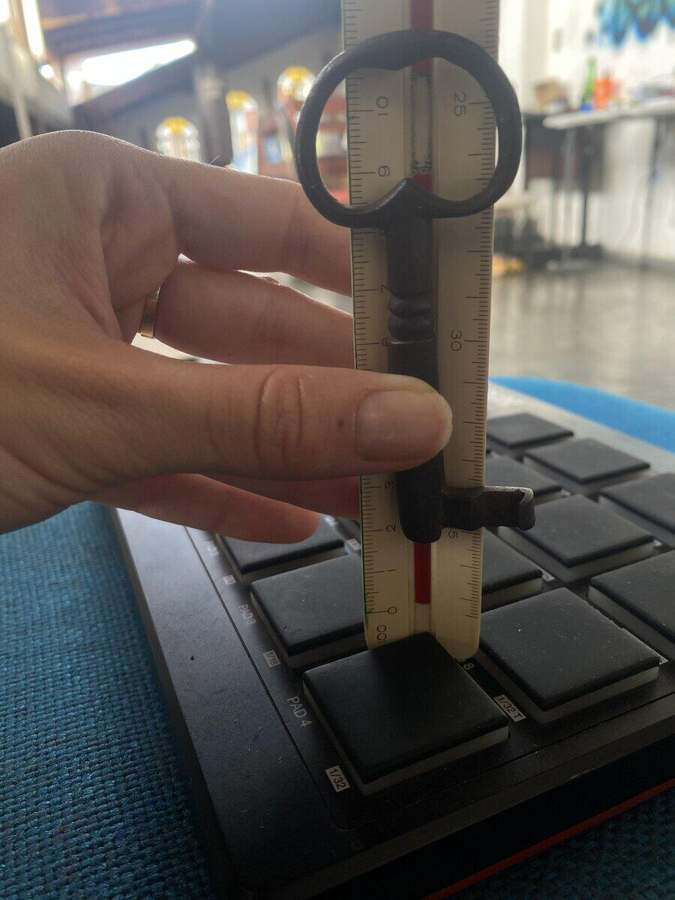
\includegraphics[width=\linewidth]{Imagens/Fotos/ensaio_queda_39g.jpg}
\end{minipage}
\caption{Ensaio com corpo de massa conhecida: aferição da massa de 39~g, à esquerda, e posicionamento do corpo em relação ao pad e à régua de referência, à direita}
\label{fig:ensaio_queda_massa}
\legend{Fonte: Elaboração própria (2026).}
\end{figure}


A escolha dessa faixa foi precedida por ensaios exploratórios, a partir dos quais a faixa utilizada na coleta definitiva foi limitada a 5~cm.

Mantendo-se constante a massa do corpo, a altura de queda foi utilizada como variável de controle da energia potencial gravitacional imediatamente antes da liberação. Para cada condição foram calculadas a energia potencial e a velocidade teórica de impacto, desconsiderando perdas por resistência do ar, por meio de

\begin{equation}
E_p = mgh
\end{equation}

e

\begin{equation}
v = \sqrt{2gh},
\end{equation}

em que $m$ representa a massa do corpo, $g$ a aceleração da gravidade e $h$ a altura de queda. Essas grandezas foram empregadas apenas para caracterizar as condições do ensaio. A força de impacto não foi calculada, pois depende também do tempo e das condições de contato entre o corpo e o pad.

Para este ensaio específico, o programa de aquisição utilizou um mapeamento linear entre a faixa útil de \textit{velocity} MIDI, de 1 a 127, e a faixa de PWM de 80 a 255. Essa escolha permitiu explorar a faixa dinâmica completa do controlador durante a caracterização. O mapeamento empregado no programa de teste foi definido por

\begin{equation}
P_{\mathrm{PWM}} =
80 +
\frac{V_{\mathrm{MIDI}}-1}{126}
\left(255-80\right),
\label{eq:mapeamento_ensaio_queda}
\end{equation}

para $1 \leq V_{\mathrm{MIDI}} \leq 127$, com arredondamento para o valor inteiro mais próximo.

\subsubsection{Filtragem dos repiques}
\label{sec:filtragem_repiques}

Eventos secundários produzidos por repiques após o primeiro contato do corpo com o pad não representam novas quedas independentes e poderiam introduzir repetições artificiais na série experimental.

Para evitar esse efeito, cada repetição foi iniciada manualmente no programa antes da liberação do corpo. Ao ser armada uma nova repetição, os eventos MIDI pendentes eram descartados e o software passava a aguardar o primeiro evento \texttt{note\_on} válido proveniente do pad selecionado. Esse primeiro evento era registrado como impacto principal.

Após o registro, foi aberta uma janela temporal de 0,60~s. Eventos adicionais do mesmo pad ocorridos nesse intervalo foram classificados como repiques e desconsiderados na determinação da \textit{velocity} e do PWM da repetição. A quantidade de eventos descartados permaneceu registrada no arquivo CSV, permitindo verificar posteriormente a ocorrência do fenômeno sem incorporá-lo como uma nova observação experimental.

Ao final da coleta foram calculados, para cada altura, média, mediana, desvio-padrão, valores mínimo e máximo de \textit{velocity} e PWM. A associação entre a altura de queda e a resposta do controlador foi avaliada principalmente pelo coeficiente de correlação de Spearman, adequado à verificação de uma tendência monotônica sem exigir linearidade estrita entre as variáveis.


\subsection{Ensaio Acústico do Atuador em Função do PWM}
\markright{Metodologia}
\label{sec:ensaio_acustico_pwm}

Foi realizado um segundo ensaio com o objetivo de verificar se a alteração do comando PWM produzia mudanças mensuráveis na frequência associada ao funcionamento do motor Vibracall 1027.

O ESP32 foi comandado diretamente por UDP utilizando seis valores de PWM: 80, 115, 150, 185, 220 e 255. Cada condição permaneceu ativa durante 8~s, seguida por um intervalo de 2~s com o motor desligado. A sequência completa foi repetida três vezes, resultando em 18 blocos de acionamento.

A automatização do ensaio permitiu registrar em arquivo CSV os instantes de início e término de cada bloco, possibilitando relacionar posteriormente os trechos da gravação ao valor PWM correspondente. O som produzido durante o funcionamento do atuador foi registrado com um microfone condensador em arquivo WAV, com taxa de amostragem de 44,1~kHz e resolução de 24~bits.

A configuração física utilizada durante a gravação é apresentada na Figura~\ref{fig:ensaio_microfone_condensador}. O motor e o microfone foram mantidos em posições fixas durante a sequência, de modo a reduzir alterações de distância e orientação entre os níveis de PWM avaliados.

\begin{figure}[!htbp]
\centering
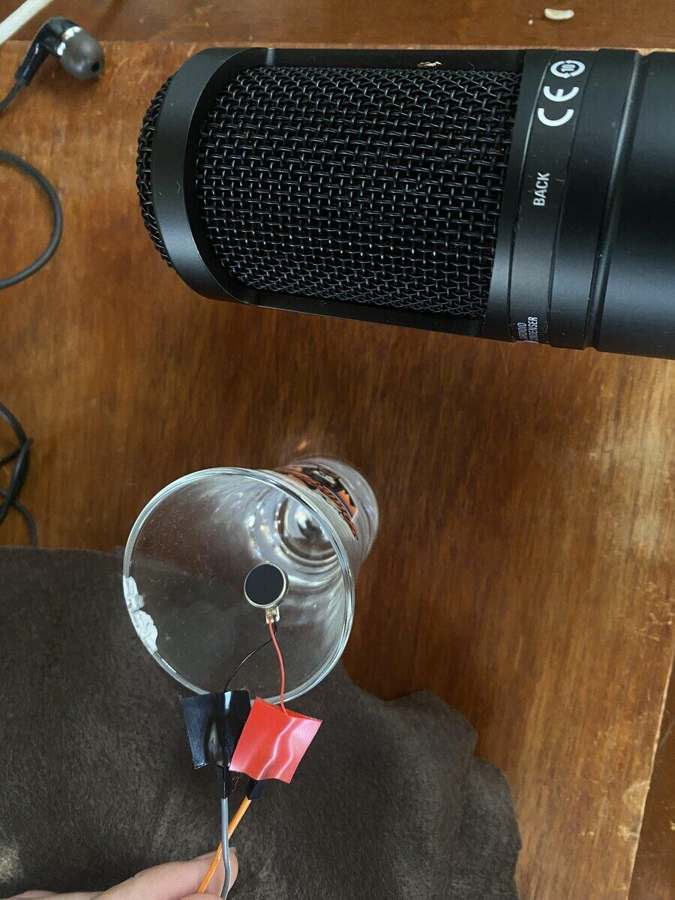
\includegraphics[
width=0.55\linewidth,
keepaspectratio
]{Imagens/Fotos/ensaio_microfone.jpg}
\caption{Configuração experimental utilizada na caracterização acústica do motor com microfone condensador}
\label{fig:ensaio_microfone_condensador}
\legend{Fonte: Elaboração própria (2026).}
\end{figure}


A análise foi realizada no domínio da frequência. Para cada bloco de acionamento foi considerada a região de funcionamento estabelecido do motor, evitando-se as transições de partida e desligamento. A componente tonal de baixa frequência associada ao atuador foi então identificada no espectro de cada trecho. Componentes estacionárias que não acompanharam a variação do PWM foram desconsideradas na determinação da frequência representativa do motor.

Foram calculadas a média, o desvio-padrão e o coeficiente de variação das três repetições para cada valor PWM. Também foram determinados os coeficientes de correlação de Pearson e de Spearman entre o comando aplicado e a frequência acústica identificada.

Esse procedimento fornece uma medida indireta do comportamento dinâmico do motor. Como a grandeza foi obtida por captação acústica, os valores não correspondem a uma medição direta da aceleração, do deslocamento ou da amplitude mecânica da vibração.


\subsection{Validação da Alimentação Embarcada}

Após a validação do circuito utilizando alimentação de bancada, foi realizada a integração do sistema de alimentação destinado à operação autônoma da unidade vestível.

Foram utilizadas duas células recarregáveis de íons de lítio associadas em configuração 2S, juntamente com um módulo BMS e um conversor DC--DC baseado no MP1584EN.

Antes da conexão ao ESP32, a tensão de saída do conversor foi ajustada utilizando multímetro para um valor próximo de 3,3~V.

Após a conexão do circuito embarcado, foram realizadas medições diretamente no barramento de alimentação do ESP32 durante sua operação.

Também foram realizados testes de conectividade entre o computador e o ESP32 utilizando mensagens ICMP por meio do comando \texttt{ping}. Esses testes foram empregados como verificação auxiliar da permanência do microcontrolador conectado à rede durante a operação alimentada pelas baterias.

\subsection{Validação do Feedback Visual}

Após a validação do canal vibrotátil e da alimentação embarcada, foi incorporado ao protótipo um LED de alto brilho destinado à geração do feedback visual.

O LED foi conectado ao GPIO 21 do ESP32 por meio de um resistor de 220~$\Omega$, utilizado para limitar a corrente fornecida ao componente.

O firmware do microcontrolador foi modificado para aplicar ao LED o mesmo valor PWM recebido para o controle do canal vibrotátil.

Inicialmente, o funcionamento do canal visual foi avaliado por meio do envio direto de comandos UDP.

Posteriormente, foram utilizados valores PWM diferentes para verificar a capacidade de modificar o nível de acionamento do LED a partir do mesmo parâmetro utilizado para o controle vibrotátil.


\subsection{Validação Integrada da Arquitetura}

A etapa final dos procedimentos experimentais consistiu na operação integrada dos principais módulos da arquitetura desenvolvida.

O ensaio foi realizado utilizando a cadeia formada pelo controlador MIDI Akai MPD218, computador com o software desenvolvido em Python, comunicação UDP sobre rede Wi-Fi, microcontrolador ESP32, estágio eletrônico de acionamento, motor Vibracall 1027, LED de alto brilho e sistema de alimentação embarcado.

Durante a interação com os pads, os eventos MIDI foram capturados pelo software e seus respectivos valores de \textit{velocity} foram processados para determinação do comando PWM.

Os comandos foram transmitidos ao ESP32, que aplicou o mesmo valor de controle ao canal vibrotátil associado ao GPIO 18 e ao canal visual associado ao GPIO 21.

Também foi utilizada a interface gráfica desenvolvida no computador para acompanhar os eventos MIDI, o pad acionado, o valor de \textit{velocity} e o valor PWM calculado durante a execução.

Os resultados obtidos durante esses procedimentos são apresentados e discutidos no Capítulo 5.

\section{Critérios de Validação}
\markright{Metodologia}
\label{sec:criterios_validacao}

A validação considerou o funcionamento individual dos módulos e sua integração. Na aquisição MIDI, verificou-se a identificação de eventos e a extração da \textit{velocity}; no processamento, a relação monotônica entre valores crescentes de entrada e comandos PWM, respeitados os limites mínimo e máximo definidos. Para a comunicação UDP, foram comparados os identificadores e as quantidades de pacotes transmitidos e recebidos, além de seus registros temporais.

A avaliação eletrônica considerou a capacidade do ESP32 de comandar o MOSFET e o motor, bem como a resposta do LED aos comandos de acionamento, desligamento e variação de PWM. Na alimentação, verificou-se a operação do microcontrolador conectado à rede Wi-Fi utilizando baterias, BMS e conversor DC--DC, sem alimentação USB. A validação integrada exigiu a propagação de um evento MIDI até as saídas vibrotátil e visual, com a unidade embarcada alimentada localmente.

No ensaio de queda, a evidência de resposta foi a tendência monotônica entre altura e \textit{velocity}, considerando a dispersão dos registros e excluindo repiques conforme o procedimento estabelecido. No ensaio acústico, foram comparadas as frequências identificadas para níveis crescentes de PWM, com suas variações entre repetições. As simulações elétricas foram examinadas separadamente, pela resposta do modelo com e sem diodo de \textit{flyback} e para diferentes razões cíclicas.

Esses critérios avaliam a viabilidade técnica, não a equivalência perceptiva das modalidades. Os resultados são discutidos no Capítulo 5.
